\documentclass[]{article}

\usepackage{xargs} 
\usepackage[colorinlistoftodos,prependcaption,textsize=tiny]{todonotes}
\newcommandx{\unsure}[2][1=]{\todo[linecolor=red,backgroundcolor=red!25,bordercolor=red,#1]{#2}}
\newcommandx{\change}[2][1=]{\todo[linecolor=blue,backgroundcolor=blue!25,bordercolor=blue,#1]{#2}}
\newcommandx{\info}[2][1=]{\todo[linecolor=OliveGreen,backgroundcolor=OliveGreen!25,bordercolor=OliveGreen,#1]{#2}}
\newcommandx{\improvement}[2][1=]{\todo[linecolor=purple,backgroundcolor=purple!25,bordercolor=purple,#1]{#2}}
\newcommandx{\thiswillnotshow}[2][1=]{\todo[disable,#1]{#2}}

\usepackage{enumitem}
\usepackage{multicol}

\usepackage{graphicx}
\usepackage{caption}
\usepackage{subcaption}

%opening
\title{}
\author{}

\begin{document}

\maketitle

\begin{abstract}

\end{abstract}

\section{Introduction}

\section{Related Work}

\section{Experiment Setup}

\todo{put a picture of the experiment setup here}

The multitouch user interface device used in this experiment is a 3M \todo{Exact model here} screen. 
This screen can track up to 20 simultaneous points, but reports only points, rather than shapes or areas of contact. \todo{pressure information? I think I had this in my initial drawing scripts}


\subsection{Experiment Conditions}

Users were given tasks in one of five conditions, varying by how many robots were in each condition. 
The conditions consisted of 1-2 robots, 10 robots, 100 robots, 1000 robots, or an unknown number of robots, represented by a cloud. 
For each condition, the user was requested to perform a sequence of tasks. 
The exact number of tasks varied between conditions due to some tasks not making sense with the number of robots involved. 



\section{Analysis}

\subsection{Participant Demographics}

\section{Conclusions}

\bibliography{../proposal/swarm.bib}
\bibliographystyle{apalike}

\section{Appendix of all Test Slides}
\begin{figure}
	\centering
	\begin{subfigure}{0.42\textwidth}
		\centering
		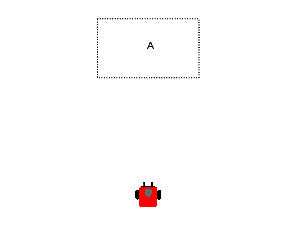
\includegraphics[width=\linewidth]{slide_images/Swarm_Robot_Control_-_Single_Robot_0003.png}
		\caption{Move to A}
		\label{fig:sub1}
	\end{subfigure}%
	\begin{subfigure}{0.42\textwidth}
		\centering
		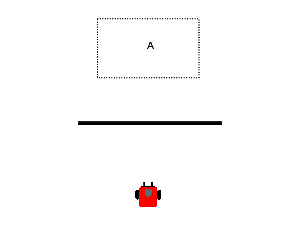
\includegraphics[width=\linewidth]{slide_images/Swarm_Robot_Control_-_Single_Robot_0005.png}
		\caption{Move to A with wall}
		\label{fig:sub2}
	\end{subfigure}
	\begin{subfigure}{0.42\textwidth}
		\centering
		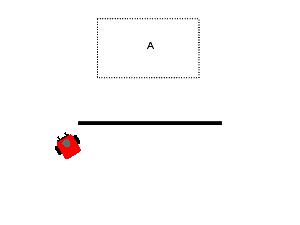
\includegraphics[width=\linewidth]{slide_images/Swarm_Robot_Control_-_Single_Robot_0007.png}
		\caption{Stop the robot}
		\label{fig:sub1}
	\end{subfigure}%
	\begin{subfigure}{0.42\textwidth}
		\centering
		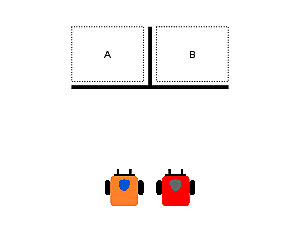
\includegraphics[width=\linewidth]{slide_images/Swarm_Robot_Control_-_Single_Robot_0009.png}
		\caption{Orange to B, Red to A}
		\label{fig:sub2}
	\end{subfigure}
	\begin{subfigure}{0.42\textwidth}
		\centering
		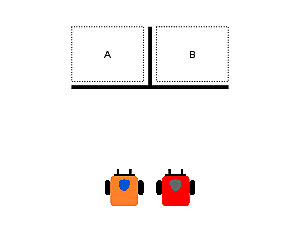
\includegraphics[width=\linewidth]{slide_images/Swarm_Robot_Control_-_Single_Robot_0011.png}
		\caption{Orange to A, Red to B}
		\label{fig:sub1}
	\end{subfigure}%
	\begin{subfigure}{0.42\textwidth}
		\centering
		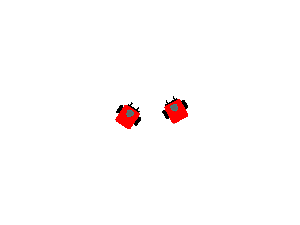
\includegraphics[width=\linewidth]{slide_images/Swarm_Robot_Control_-_Single_Robot_0013.png}
		\caption{Divide group}
		\label{fig:sub2}
	\end{subfigure}
	\begin{subfigure}{0.42\textwidth}
		\centering
		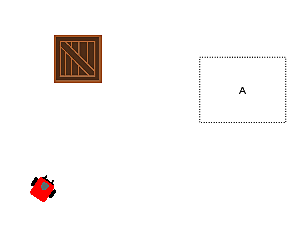
\includegraphics[width=\linewidth]{slide_images/Swarm_Robot_Control_-_Single_Robot_0015.png}
		\caption{Move the crate to A}
		\label{fig:sub1}
	\end{subfigure}%
	\begin{subfigure}{0.42\textwidth}
		\centering
		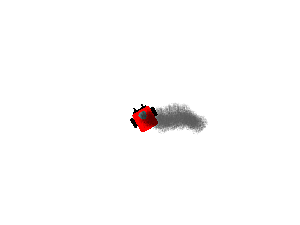
\includegraphics[width=\linewidth]{slide_images/Swarm_Robot_Control_-_Single_Robot_0017.png}
		\caption{Mark defective robot}
		\label{fig:sub2}
	\end{subfigure}
	\label{fig:single_robot_slides}
\end{figure}


\begin{figure}
	\ContinuedFloat
	\centering
	\begin{subfigure}{0.42\textwidth}
		\centering
		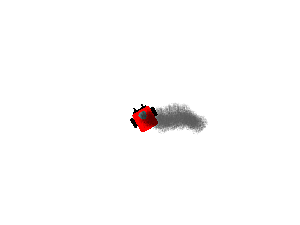
\includegraphics[width=\linewidth]{slide_images/Swarm_Robot_Control_-_Single_Robot_0019.png}
		\caption{Remove defective robot}
		\label{fig:sub1}
	\end{subfigure}%
	\begin{subfigure}{0.42\textwidth}
		\centering
		
\includegraphics[width=\linewidth]{slide_images/Swarm_Robot_Control_-_Single_Robot_0021.png}
		\caption{Patrol the screen border}
		\label{fig:sub2}
	\end{subfigure}
	\begin{subfigure}{0.42\textwidth}
		\centering
		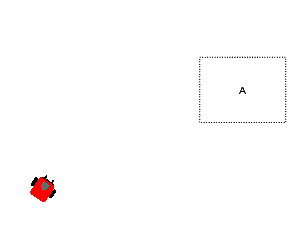
\includegraphics[width=\linewidth]{slide_images/Swarm_Robot_Control_-_Single_Robot_0023.png}
		\caption{Patrol area A}
		\label{fig:sub1}
	\end{subfigure}
	\label{fig:single_robot_slides_pt2}
\end{figure}


\begin{figure}
	\centering
	\begin{subfigure}{0.42\textwidth}
		\centering
		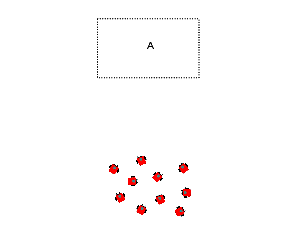
\includegraphics[width=\linewidth]{slide_images/Swarm_Robot_Control_-_10_Robot_0003.png}
		\caption{Move to A}
		\label{fig:sub1}
	\end{subfigure}%
	\begin{subfigure}{0.42\textwidth}
		\centering
		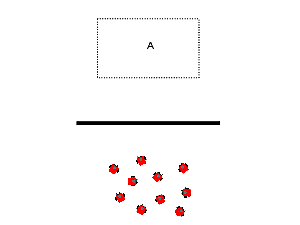
\includegraphics[width=\linewidth]{slide_images/Swarm_Robot_Control_-_10_Robot_0005.png}
		\caption{Move to A with wall}
		\label{fig:sub2}
	\end{subfigure}
	\begin{subfigure}{0.42\textwidth}
		\centering
		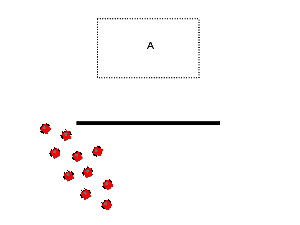
\includegraphics[width=\linewidth]{slide_images/Swarm_Robot_Control_-_10_Robot_0007.png}
		\caption{Stop the robots}
		\label{fig:sub1}
	\end{subfigure}%
	\begin{subfigure}{0.42\textwidth}
		\centering
		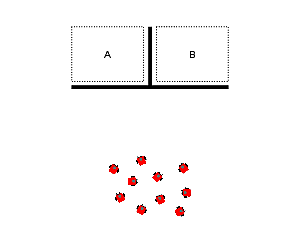
\includegraphics[width=\linewidth]{slide_images/Swarm_Robot_Control_-_10_Robot_0009.png}
		\caption{Divide around obstacle}
		\label{fig:sub2}
	\end{subfigure}
	\begin{subfigure}{0.42\textwidth}
		\centering
		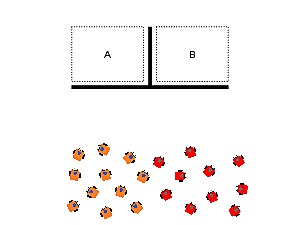
\includegraphics[width=\linewidth]{slide_images/Swarm_Robot_Control_-_10_Robot_0011.png}
		\caption{Orange to B, Red to A}
		\label{fig:sub1}
	\end{subfigure}%
	\begin{subfigure}{0.42\textwidth}
		\centering
		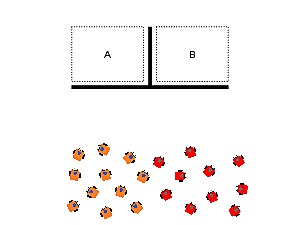
\includegraphics[width=\linewidth]{slide_images/Swarm_Robot_Control_-_10_Robot_0013.png}
		\caption{Orange to A, Red to B}
		\label{fig:sub2}
	\end{subfigure}
	\begin{subfigure}{0.42\textwidth}
		\centering
		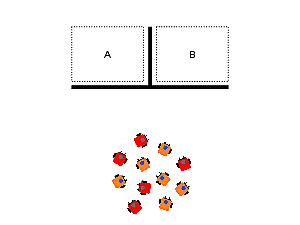
\includegraphics[width=\linewidth]{slide_images/Swarm_Robot_Control_-_10_Robot_0015.png}
		\caption{Orange to A, Red to B}
		\label{fig:sub1}
	\end{subfigure}%
	\begin{subfigure}{0.42\textwidth}
		\centering
		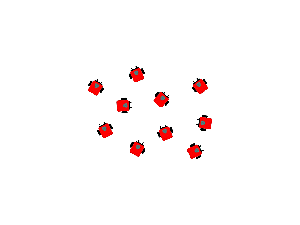
\includegraphics[width=\linewidth]{slide_images/Swarm_Robot_Control_-_10_Robot_0017.png}
		\caption{Divide group}
		\label{fig:sub2}
	\end{subfigure}
\end{figure}
	
	
\begin{figure}
	\ContinuedFloat
	\centering		
	\begin{subfigure}{0.42\textwidth}
		\centering
		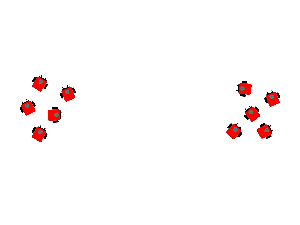
\includegraphics[width=\linewidth]{slide_images/Swarm_Robot_Control_-_10_Robot_0019.png}
		\caption{Combine groups}
		\label{fig:sub1}
	\end{subfigure}%
	\begin{subfigure}{0.42\textwidth}
		\centering
		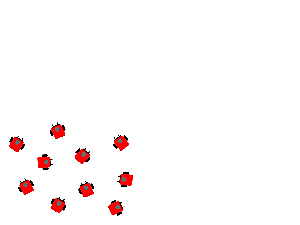
\includegraphics[width=\linewidth]{slide_images/Swarm_Robot_Control_-_10_Robot_0021.png}
		\caption{}
		\label{fig:sub2}
	\end{subfigure}
	\begin{subfigure}{0.42\textwidth}
		\centering
		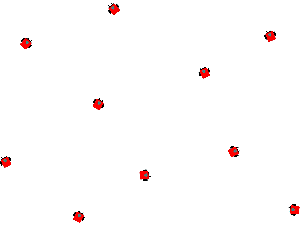
\includegraphics[width=\linewidth]{slide_images/Swarm_Robot_Control_-_10_Robot_0023.png}
		\caption{}
		\label{fig:sub1}
	\end{subfigure}%
	\begin{subfigure}{0.42\textwidth}
		\centering
		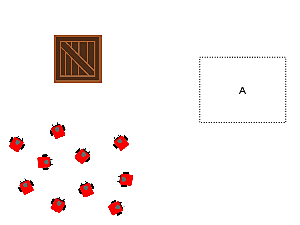
\includegraphics[width=\linewidth]{slide_images/Swarm_Robot_Control_-_10_Robot_0025.png}
		\caption{Orange to A, Red to B}
		\label{fig:sub1}
	\end{subfigure}
	\begin{subfigure}{0.42\textwidth}
		\centering
		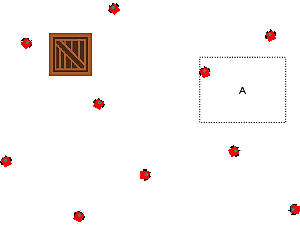
\includegraphics[width=\linewidth]{slide_images/Swarm_Robot_Control_-_10_Robot_0027.png}
		\caption{Divide group}
		\label{fig:sub2}
	\end{subfigure}%
	\begin{subfigure}{0.42\textwidth}
		\centering
		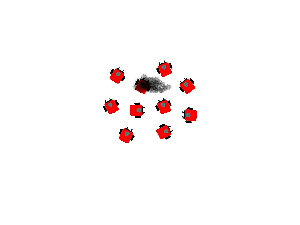
\includegraphics[width=\linewidth]{slide_images/Swarm_Robot_Control_-_10_Robot_0029.png}
		\caption{Combine groups}
		\label{fig:sub1}
	\end{subfigure}
	\begin{subfigure}{0.42\textwidth}
		\centering
		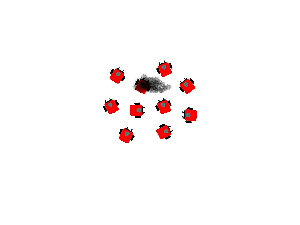
\includegraphics[width=\linewidth]{slide_images/Swarm_Robot_Control_-_10_Robot_0031.png}
		\caption{Form a line}
		\label{fig:sub2}
	\end{subfigure}%
	\begin{subfigure}{0.42\textwidth}
		\centering
		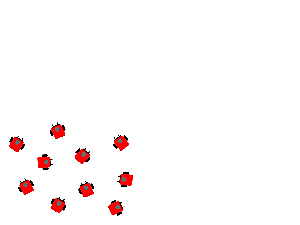
\includegraphics[width=\linewidth]{slide_images/Swarm_Robot_Control_-_10_Robot_0033.png}
		\caption{Form a square}
		\label{fig:sub1}
	\end{subfigure}
\end{figure}
	
	
\begin{figure}
	\ContinuedFloat
	\centering	
	\begin{subfigure}{0.42\textwidth}
		\centering
		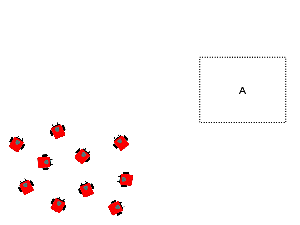
\includegraphics[width=\linewidth]{slide_images/Swarm_Robot_Control_-_10_Robot_0035.png}
		\caption{Move the crate to A}
		\label{fig:sub1}
	\end{subfigure}%
	\begin{subfigure}{0.42\textwidth}
		\centering
		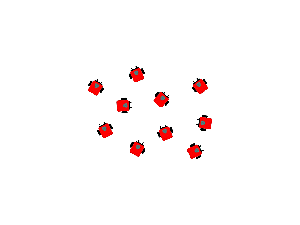
\includegraphics[width=\linewidth]{slide_images/Swarm_Robot_Control_-_10_Robot_0037.png}
		\caption{Move the crate to A}
		\label{fig:sub2}
	\end{subfigure}
	\label{fig:10_robot_slides}
\end{figure}

\begin{figure}
	\centering
	\begin{subfigure}{0.42\textwidth}
		\centering
		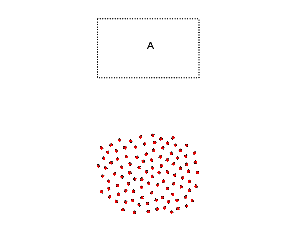
\includegraphics[width=\linewidth]{slide_images/Swarm_Robot_Control_-_100_Robot_0003.png}
		\caption{Move to A}
		\label{fig:sub1}
	\end{subfigure}%
	\begin{subfigure}{0.42\textwidth}
		\centering
		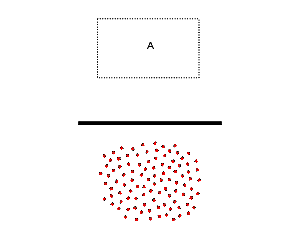
\includegraphics[width=\linewidth]{slide_images/Swarm_Robot_Control_-_100_Robot_0005.png}
		\caption{Move to A with wall}
		\label{fig:sub2}
	\end{subfigure}
	\begin{subfigure}{0.42\textwidth}
		\centering
		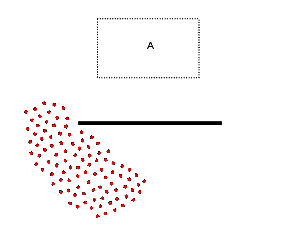
\includegraphics[width=\linewidth]{slide_images/Swarm_Robot_Control_-_100_Robot_0007.png}
		\caption{Stop the robots}
		\label{fig:sub1}
	\end{subfigure}%
	\begin{subfigure}{0.42\textwidth}
		\centering
		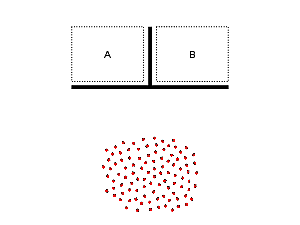
\includegraphics[width=\linewidth]{slide_images/Swarm_Robot_Control_-_100_Robot_0009.png}
		\caption{Divide around obstacle}
		\label{fig:sub2}
	\end{subfigure}
	\begin{subfigure}{0.42\textwidth}
		\centering
		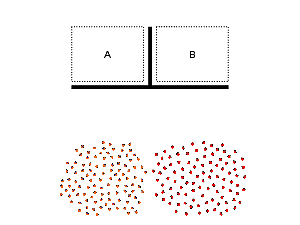
\includegraphics[width=\linewidth]{slide_images/Swarm_Robot_Control_-_100_Robot_0011.png}
		\caption{Orange to B, Red to A}
		\label{fig:sub1}
	\end{subfigure}%
	\begin{subfigure}{0.42\textwidth}
		\centering
		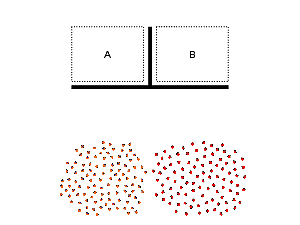
\includegraphics[width=\linewidth]{slide_images/Swarm_Robot_Control_-_100_Robot_0013.png}
		\caption{Orange to A, Red to B}
		\label{fig:sub2}
	\end{subfigure}
	\begin{subfigure}{0.42\textwidth}
		\centering
		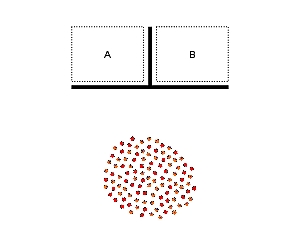
\includegraphics[width=\linewidth]{slide_images/Swarm_Robot_Control_-_100_Robot_0015.png}
		\caption{Orange to A, Red to B}
		\label{fig:sub1}
	\end{subfigure}%
	\begin{subfigure}{0.42\textwidth}
		\centering
		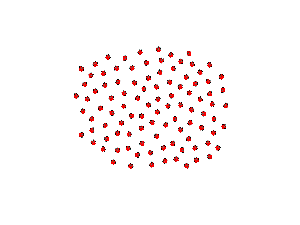
\includegraphics[width=\linewidth]{slide_images/Swarm_Robot_Control_-_100_Robot_0017.png}
		\caption{Divide group}
		\label{fig:sub2}
	\end{subfigure}
\end{figure}
\begin{figure}
	\ContinuedFloat
	\centering
	\begin{subfigure}{0.42\textwidth}
		\centering
		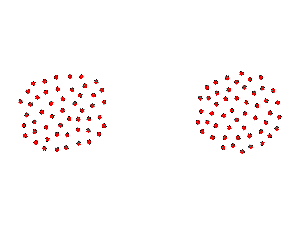
\includegraphics[width=\linewidth]{slide_images/Swarm_Robot_Control_-_100_Robot_0019.png}
		\caption{Combine groups}
		\label{fig:sub1}
	\end{subfigure}%
	\begin{subfigure}{0.42\textwidth}
		\centering
		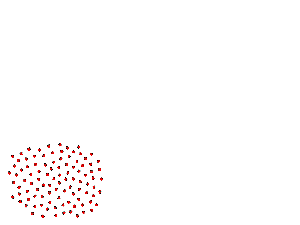
\includegraphics[width=\linewidth]{slide_images/Swarm_Robot_Control_-_100_Robot_0021.png}
		\caption{Form a line}
		\label{fig:sub2}
	\end{subfigure}
	\begin{subfigure}{0.42\textwidth}
		\centering
		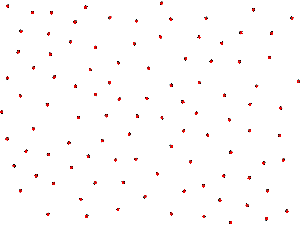
\includegraphics[width=\linewidth]{slide_images/Swarm_Robot_Control_-_100_Robot_0023.png}
		\caption{Form a square}
		\label{fig:sub1}
	\end{subfigure}%
	\begin{subfigure}{0.42\textwidth}
		\centering
		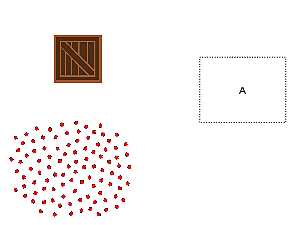
\includegraphics[width=\linewidth]{slide_images/Swarm_Robot_Control_-_100_Robot_0025.png}
		\caption{Move the crate to area A}
		\label{fig:sub1}
	\end{subfigure}
	\begin{subfigure}{0.42\textwidth}
		\centering
		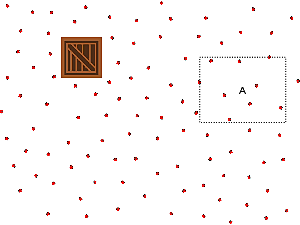
\includegraphics[width=\linewidth]{slide_images/Swarm_Robot_Control_-_100_Robot_0027.png}
		\caption{Move the crate to area A}
		\label{fig:sub2}
	\end{subfigure}%
	\begin{subfigure}{0.42\textwidth}
		\centering
		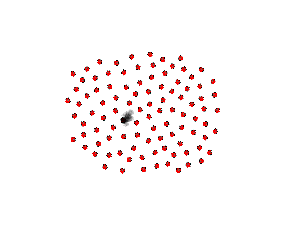
\includegraphics[width=\linewidth]{slide_images/Swarm_Robot_Control_-_100_Robot_0029.png}
		\caption{Mark defective robot}
		\label{fig:sub1}
	\end{subfigure}
	\begin{subfigure}{0.42\textwidth}
		\centering
		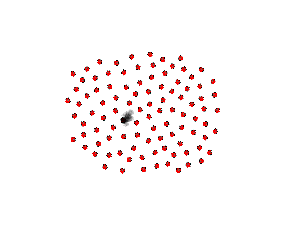
\includegraphics[width=\linewidth]{slide_images/Swarm_Robot_Control_-_100_Robot_0031.png}
		\caption{Remove defective robot}
		\label{fig:sub2}
	\end{subfigure}%
	\begin{subfigure}{0.42\textwidth}
		\centering
		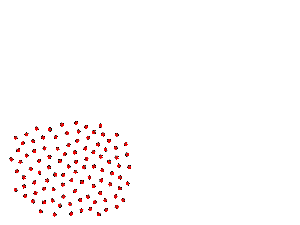
\includegraphics[width=\linewidth]{slide_images/Swarm_Robot_Control_-_100_Robot_0033.png}
		\caption{Patrol the screen border}
		\label{fig:sub1}
	\end{subfigure}
\end{figure}
\begin{figure}
	\ContinuedFloat
	\centering	
		\begin{subfigure}{0.42\textwidth}
		\centering
		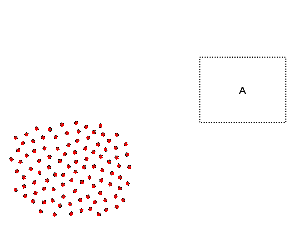
\includegraphics[width=\linewidth]{slide_images/Swarm_Robot_Control_-_100_Robot_0035.png}
		\caption{Patrol area A}
		\label{fig:sub1}
	\end{subfigure}%
	\begin{subfigure}{0.42\textwidth}
		\centering
		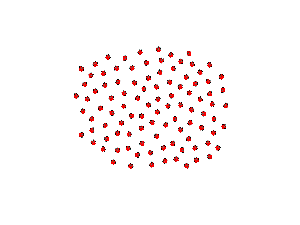
\includegraphics[width=\linewidth]{slide_images/Swarm_Robot_Control_-_100_Robot_0037.png}
		\caption{Disperse over screen}
		\label{fig:sub2}
	\end{subfigure}
	\label{fig:100_robot_slides}
\end{figure}


\begin{figure}
	\centering
	\begin{subfigure}{0.42\textwidth}
		\centering
		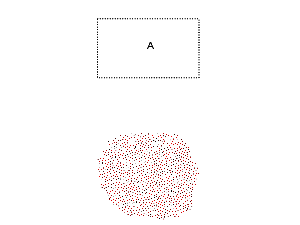
\includegraphics[width=\linewidth]{slide_images/Swarm_Robot_Control_-_1000_Robot_0003.png}
		\caption{Move to A}
		\label{fig:sub1}
	\end{subfigure}%
	\begin{subfigure}{0.42\textwidth}
		\centering
		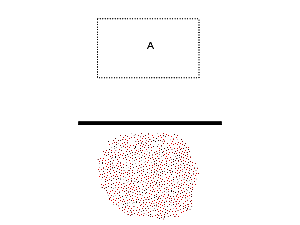
\includegraphics[width=\linewidth]{slide_images/Swarm_Robot_Control_-_1000_Robot_0005.png}
		\caption{Move to A with wall}
		\label{fig:sub2}
	\end{subfigure}
	\begin{subfigure}{0.42\textwidth}
		\centering
		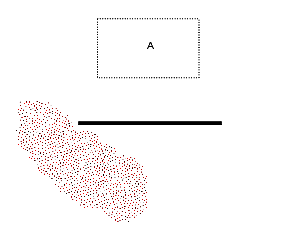
\includegraphics[width=\linewidth]{slide_images/Swarm_Robot_Control_-_1000_Robot_0007.png}
		\caption{Stop the robots}
		\label{fig:sub1}
	\end{subfigure}%
	\begin{subfigure}{0.42\textwidth}
		\centering
		\includegraphics[width=\linewidth]{slide_images/Swarm_Robot_Control_-_1000_Robot_0009.png}
		\caption{Divide around obstacle}
		\label{fig:sub2}
	\end{subfigure}
	\begin{subfigure}{0.42\textwidth}
		\centering
		\includegraphics[width=\linewidth]{slide_images/Swarm_Robot_Control_-_1000_Robot_0011.png}
		\caption{Orange to B, Red to A}
		\label{fig:sub1}
	\end{subfigure}%
	\begin{subfigure}{0.42\textwidth}
		\centering
		\includegraphics[width=\linewidth]{slide_images/Swarm_Robot_Control_-_1000_Robot_0013.png}
		\caption{Orange to A, Red to B}
		\label{fig:sub2}
	\end{subfigure}
	\begin{subfigure}{0.42\textwidth}
		\centering
		\includegraphics[width=\linewidth]{slide_images/Swarm_Robot_Control_-_1000_Robot_0015.png}
		\caption{Orange to A, Red to B}
		\label{fig:sub1}
	\end{subfigure}%
	\begin{subfigure}{0.42\textwidth}
		\centering
		\includegraphics[width=\linewidth]{slide_images/Swarm_Robot_Control_-_1000_Robot_0017.png}
		\caption{Divide group}
		\label{fig:sub2}
	\end{subfigure}
\end{figure}
\begin{figure}
	\ContinuedFloat
	\centering
	\begin{subfigure}{0.42\textwidth}
		\centering
		\includegraphics[width=\linewidth]{slide_images/Swarm_Robot_Control_-_1000_Robot_0019.png}
		\caption{Combine groups}
		\label{fig:sub1}
	\end{subfigure}%
	\begin{subfigure}{0.42\textwidth}
		\centering
		\includegraphics[width=\linewidth]{slide_images/Swarm_Robot_Control_-_1000_Robot_0021.png}
		\caption{Form a line}
		\label{fig:sub2}
	\end{subfigure}
	\begin{subfigure}{0.42\textwidth}
		\centering
		\includegraphics[width=\linewidth]{slide_images/Swarm_Robot_Control_-_1000_Robot_0023.png}
		\caption{Form a square}
		\label{fig:sub1}
	\end{subfigure}%
	\begin{subfigure}{0.42\textwidth}
		\centering
		\includegraphics[width=\linewidth]{slide_images/Swarm_Robot_Control_-_1000_Robot_0025.png}
		\caption{Move the crate to area A}
		\label{fig:sub1}
	\end{subfigure}
	\begin{subfigure}{0.42\textwidth}
		\centering
		\includegraphics[width=\linewidth]{slide_images/Swarm_Robot_Control_-_1000_Robot_0027.png}
		\caption{Move the crate to area A}
		\label{fig:sub2}
	\end{subfigure}%
	\begin{subfigure}{0.42\textwidth}
		\centering
		\includegraphics[width=\linewidth]{slide_images/Swarm_Robot_Control_-_1000_Robot_0029.png}
		\caption{Mark defective robot}
		\label{fig:sub1}
	\end{subfigure}
	\begin{subfigure}{0.42\textwidth}
		\centering
		\includegraphics[width=\linewidth]{slide_images/Swarm_Robot_Control_-_1000_Robot_0031.png}
		\caption{Remove defective robot}
		\label{fig:sub2}
	\end{subfigure}%
	\begin{subfigure}{0.42\textwidth}
		\centering
		\includegraphics[width=\linewidth]{slide_images/Swarm_Robot_Control_-_1000_Robot_0033.png}
		\caption{Patrol the screen border}
		\label{fig:sub1}
	\end{subfigure}
\end{figure}
\begin{figure}
	\ContinuedFloat
	\centering	
		\begin{subfigure}{0.42\textwidth}
		\centering
		\includegraphics[width=\linewidth]{slide_images/Swarm_Robot_Control_-_1000_Robot_0035.png}
		\caption{Patrol area A}
		\label{fig:sub1}
	\end{subfigure}%
	\begin{subfigure}{0.42\textwidth}
		\centering
		\includegraphics[width=\linewidth]{slide_images/Swarm_Robot_Control_-_1000_Robot_0037.png}
		\caption{Disperse over screen}
		\label{fig:sub2}
	\end{subfigure}
	\label{fig:1000_robot_slides}
\end{figure}

\end{document}
